\documentclass[12pt]{article}

\pagenumbering{gobble}
\linespread{1.2}

\usepackage{fancyhdr}
\usepackage[headheight=0.5in,margin=1in]{geometry}
\usepackage{graphicx}

\setlength{\parindent}{0in}

\begin{document}
    \pagestyle{fancy}

    \fancyhead[L]{Software Requirements Specification \\ Group 1}
    \fancyhead[R]{Alex Agruso, Mauro Alvizo Jr. \\ Daniel Arreguin, Jake Bram}

    \section{Introduction}

    \subsection{Project Scope}

    Our program will be a simple powder-toy physics simulator. It will be a
    standalone desktop application written in C++ using the SFML multimedia
    library. The UI will consist
    of a grid of pixels, with each pixel represent a different simulated
    particles. Each particle has an element which determines how it interacts
    with other particles. The user will be able to add and remove particles from
    the board and watch the physics simulation unfold.

    \section{Functional Requirements}

    \subsection{User Interface}

    The user interface will consist primarily of two sections: element
    selection, and the game board.
    Users will be able to choose which element they would like to use by
    clicking its respective button.
    Next, they will click and drag on the game board which will add particles of
    that element to the screen.
    The physics simulation runs continuously, unless the user decides to pause
    it.
    Finally, the user will be able to save and load board layouts, saving a
    currently running simulation for later.

    \subsection{Particles and Elements}
    
    Physics interactions occur between particles, with each particle being of a
    certain element.
    A particle's element determines how it interacts with other particles.
    
    \subsubsection{Element Classes}

    There are four primary classes of elements: solids, liquids, gasses, and powders.
    Each is described as follows:

    \textbf{Solid:} Static and rigid; is not affected by gravity.

    \textbf{Liquid:} Dynamic; flows freely but is affected by gravity and
    collides with other particles.
    
    \textbf{Gas:} Dynamic; diffuses evenly, is not affected by gravity but still
    collides with other particles.

    \textbf{Powder:} Dynamic; forms piles, is affected by gravity, and collides
    with other particles.

    \vspace{0.5cm}

    We currently plan on implementing 20 different elements, with interactions
    documented in the following sections.

    \subsubsection{Solid Elements}

    \textbf{Wall:} Is indestructible and does not interact with other elements.
    Purely serves as a collision boundary.

    \textbf{Metal:} Can be melted by lava, and can be electrified using spark.
    Electrified metal can also ignite TNT and gunpowder.

    \textbf{Wood:} Can be burned by fire or lava, producing smoke.

    \textbf{Glass:} Produced when sand touches lava. Produces stone when
    destroyed with TNT or gunpowder.
    
    \textbf{TNT:} Explodes when touching fire, lava, or electrified metal.
    Destroys most materials.

    \textbf{Plant:} Can be burned by fire or lava, producing smoke.
    Grows like an amoeba if in contact with wood.

    \textbf{Rock:} Can be melted bny lava, and produces stone when destroyed
    with TNT or gunpowder.

    \subsubsection{Liquid Elements}

    \textbf{Water:} Puts out fire, producing steam. Also cools lava into stone.
    Freezes when contacting ice.

    \textbf{Lava:} Very hot, ignites anything that is flammable. Cools into
    stone when contacting cold objects.

    \textbf{Poison:} Flammable, corrupts plant into more poison.

    \textbf{Oil:} Flammable, floats on top of water.

    \subsubsection{Gas Elements}

    \textbf{Smoke:} Produced by several elements when burned.

    \textbf{Fire:} Ignites anything that is flammable. Can be put out using water.

    \textbf{Steam:} Produced when water evaporates.

    \textbf{Gas Vapor:} Flammable, passively produced by oil.

    \subsubsection{Powder Elements}

    \textbf{Stone:} Melts when contacting lava.

    \textbf{Sand:} Turns into glass when in contact with fire or lava.

    \textbf{Gunpowder:} Explosive, can be ignited by fire and lava, as well as
    electrified metal.

    \textbf{Ice:} Very cold, freezes things upon contact.

    \subsubsection{Miscellaneous Elements}

    \textbf{Spark:} Can be used to electrify metal.

    \section{Non-Functional Requirements}

    \subsection{Event System}

    Our program will be built on an event system.
    Any interaction between different components of the program will be handled
    as an event.
    There will be many different types of events for our application, many of
    which will have no common functionality with each other.
    In order to limit unnecessary abstraction, we will implement the events as
    an algebraic data type using \verb|std::variant|.
    We will also use pattern matching with \verb|std::visit|.

    \subsection{Physics Engine}

    For stability, the physics engine will be limited to running at 60 ticks per
    second.
    Each particle will be represented as an instance of \verb|std::optional|
    wrapping a particle physics instance. If the particle is empty, or air, it
    takes the type of \verb|std::nullopt|, while if it is not empty, it takes
    the type of a standard physics particle. The engine will be single-threaded,
    but a multi-threaded implementation will be considered if performance is an
    issue.

    \subsubsection{Simulation Size} The physics engine should be able to fulfill
    the above requirements for a simulation that is 800 pixels wide and 600
    pixels tall.

    \subsection{Platform Compatibility}

    Our application should be able to run on Windows, Mac, and Linux.
    It should be able to run on any system with more than 2GB of memory and a
    multi-core processor.

    \section{Sequence Diagram}

    \begin{center}
        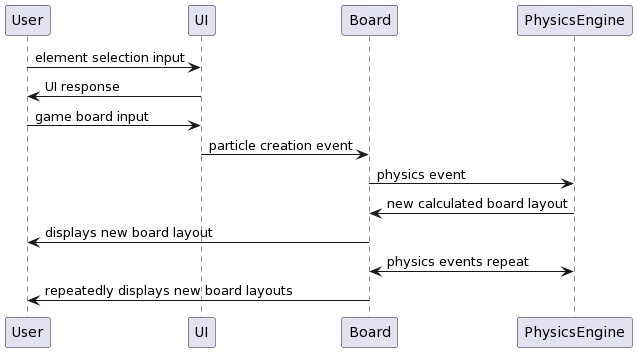
\includegraphics[scale=0.7]{sequence.png}
    \end{center}

    \section{Use Cases}

    \subsection{Element Selection}

    \textbf{Description:} User selects an element.

    \textbf{Events:} On the user click, a mouse event is created which is
    registered by the application. The button then reacts to the event and
    changes state. Finally, the game board is updated to have the current
    element that the user has specified.

    \subsection{Particle Creation}

    \textbf{Description:} User creates particles on the game board.

    \textbf{Events:} When the user clicks and drags on the game board, mouse
    events will be continuously sent to the game board. These events tell the
    game board to create new particles where the user's mouse is.

    \textbf{Exceptions:} If the specific pixel is already occupied by another
    particle, then the game board will not overwrite with the user's element.
    
\end{document}